\section{Définitions}

\begin{definition}
Un \MotDefinition{cercle}{} de centre $O$ est l'ensemble des points situés à la même distance du point $O$.

Cette distance est le \MotDefinition{rayon}{} du cercle.
\end{definition}

\vspace{2em}

\begin{tabular}{|p{.2\linewidth}|p{.46\linewidth}|p{.22\linewidth}|}
\hline
\multirow{4}{*}{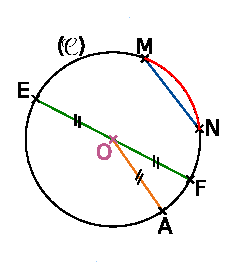
\includegraphics[width=\linewidth]{cCD01}} & Un \textbf{rayon} d'un cercle est un segment ayant pour extrémités le centre et un point de ce cercle. & Le segment $[OA]$ est un \textbf{rayon} du cercle $(\mathcal{C})$.  \\ \cline{2-3}
     & Un \MotDefinition{diamètre}{} d'un cercle est un segment ayant pour extrémités deux points de ce cercle et contenant son centre. & Le segment $[EF]$ est un \textbf{diamètre} du cercle $(\mathcal{C})$. \\ \cline{2-3}
     & Une \MotDefinition{corde}{} d'un cercle est un segment ayant pour extrémités deux points de ce cercle. & Le segment $[MN]$ est une \textbf{corde} du cercle $(\mathcal{C})$. \\ \cline{2-3}
     & Un \MotDefinition{arc de cercle}{} est une portion de cercle comprise entre deux points de ce cercle. & La portion de cercle $\overset{\frown}{MN}$ comprise entre $M$ et $N$ est un \textbf{arc du cercle} $(\mathcal{C})$. \\ \hline
     & Un \MotDefinition{disque}{} est une région du plan limitée par un cercle. &  \\ \cline{2-3}
     & Un \MotDefinition{secteur circulaire}{} est une partie du disque comprise entre deux rayons. &  \\ \hline
\end{tabular}

 
\begin{remarque}
Par commodité de langage, on appelle \og rayon \fg la longueur du rayon d'un cercle, et on appelle \og diamètre \fg la longueur de son diamètre.
\end{remarque}

\begin{remarque}
Le diamètre d'un cercle est égal au double de son rayon.
\end{remarque}




\section{Périmètre du cercle}



\begin{definition}
Le \MotDefinition{périmètre (ou circonférence)}{} d'un cercle est \textbf{la longueur de son contour}.
\end{definition} 


\begin{propriete}
Si $R$ est le rayon d’un cercle et $D$ son diamètre, la circonférence du cercle est donnée par la formule :
\[ C = 2\cdot \pi \cdot R = \pi \cdot D \qquad \qquad \text{où } \pi= 3,1415926... \]
\end{propriete}



\begin{remarque}
Comme $\pi$ est un nombre infini, on utilise souvent, pour les calculs des valeurs approchées de $\pi$. L' approximation la plus fréquente est $\boldsymbol{\pi \approx 3,14}$.
\end{remarque}


\begin{exemple*1}
Le diamètre d'un cercle mesure 3 cm. Combien mesure sa circonférence ?

On prendra $\pi \approx 3,14$.
\correction
$C = \pi  \times D = 3,14 \times 3 = 9,42$. La circonférence du cercle est 9,42\,cm.
\end{exemple*1}


\begin{exemple*1}
Le rayon d'un cercle mesure 2\,cm. Combien mesure sa circonférence ?

On prendra $\pi \approx 3,14$.
\correction
 $C = 2 \times \pi \times R = 2 \times 3,14 \times 2 = 12,56$. La circonférence mesure 12,56\,cm.
\end{exemple*1}




\begin{exemple*1}
La circonférence d'un cercle est de 15,7\,cm. Quel en est le diamètre ?
\correction
$C = \pi \times D$ donc $15,7 = 3,14 \times D$ d'où on tire $D = 15,7 \div 3,14 = 5$.

Le diamètre mesure 5\,cm.
\end{exemple*1}
 	 

		
		
		
\section{Aire du disque}



\begin{propriete}
L'\MotDefinition{aire d'un disque}{} de rayon $R$ est donnée par la formule :
\[ \mathcal{A} = \pi \times R \times R = \pi R^2 \]
\end{propriete} 
 

\begin{exemple*1}
Calculer l'aire $\mathcal{A}$ d'un disque de rayon $4,8$\,dm. Donner la valeur arrondie au cm\up{2}.
\correction
$A = \pi R^2 = \pi \times 4,82 = 3,14 \times 23,04 \approx 72,345$.

L'aire du disque est donc égale à 7 235\,cm\up{2}. 
\end{exemple*1}




\section{Calculer une aire par découpage}


\begin{exemple*1}
Calculer l’aire de la figure suivante :

\begin{center}
    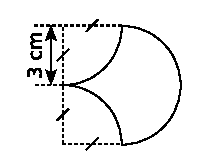
\includegraphics[width=.2\linewidth]{cCD02}
\end{center}

\correction
Pour calculer l'aire de cette figure, on découpe la figure en trois morceaux puis on les déplace pour reconstituer une figure connue.

\begin{center}
    \hfill 
\includegraphics[width=.15\linewidth]{cCD03} \hfill 
\includegraphics[width=.15\linewidth]{cCD04} \hspace*{\fill}
\end{center}
						
Calculer l'aire de cette figure revient donc à calculer l'aire d'un rectangle de largeur 3\,cm et de longueur 6\,cm : $\mathcal{A} = 3 \text{cm} \times 6 \text{cm} = 18$\,cm\up{2}.

L'aire de cette figure est 18\,cm\up{2}.
\end{exemple*1}



\begin{exemple*1}
Calculer l'aire de la figure suivante.
\begin{center}
    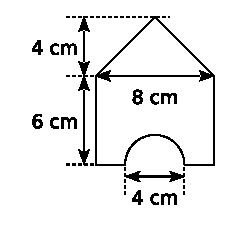
\includegraphics[width=.25\linewidth]{cCD05}
\end{center}
\correction
Pour calculer l'aire de cette figure, on repère des figures simples qui la constituent...
\begin{center}
    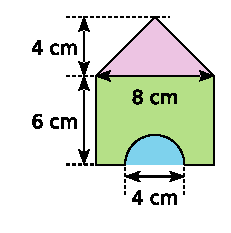
\includegraphics[width=.25\linewidth]{cCD06}
\end{center}
... puis on calcule l'aire de chacune des figures simples trouvées.

\vspace{1em}

\begin{tabular}{p{.32\linewidth}|p{.32\linewidth}|p{.32\linewidth}}
Un \textbf{triangle} dont un côté mesure 8\,cm et la hauteur relative à ce côté mesure 4\,cm. & Un \textbf{rectangle} de largeur 6\,cm et de longueur 8\,cm. & Un \textbf{demi-disque} de rayon 2\,cm. \\
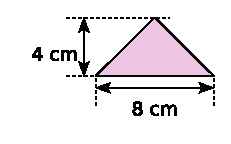
\includegraphics[width=.7\linewidth]{cCD07} & 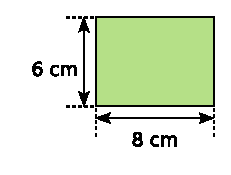
\includegraphics[width=.7\linewidth]{cCD08} & \hspace*{.3\linewidth}
\includegraphics[width=.3\linewidth]{cCD09}\\
  $\mathcal{A}_T = \dfrac{8 \times 4}{2}= 16$\,cm\up{2} & $\mathcal{A}_R = 6 \times 8 = 48$\,cm\up{2} & $\mathcal{A}_D =\dfrac{\pi \times 2^2}{2}= 2\pi$\,cm\up{2} \\
\end{tabular}

\vspace{1em}

L'aire de la figure est obtenue en additionnant l'aire du triangle et du rectangle puis en retranchant au résultat l'aire du demi-disque :
\[ \mathcal{A}= \mathcal{A}_T + \mathcal{A}_R - \mathcal{A}_D = 16 \text{ cm\up{2}} + 48 \text{ cm\up{2}} - 2\pi \text{ cm\up{2}} = 64 - 2\pi \text{ cm\up{2}}. \]

L'aire exacte de cette figure est $64 - 2\pi$\,cm\up{2}.

En prenant 3,14 comme valeur approchée du nombre $\pi$, on obtient $\mathcal{A} \approx 57,72$\,cm\up{2}.
\end{exemple*1}



\begin{exemple*1}
Calculer l'aire de chacune des figures suivantes :
\begin{center}
    \hfill 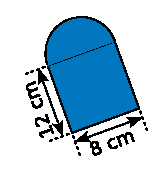
\includegraphics[width=.2\linewidth]{cCD10} \hfill 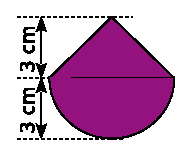
\includegraphics[width=.2\linewidth]{cCD11} \hspace*{\fill}
\end{center}
%\correction

\end{exemple*1}

							
